\documentclass[11pt]{article}

\usepackage[margin=1in]{geometry}
\usepackage{microtype}
\usepackage{hyperref}
\usepackage{enumitem}
\usepackage{amsmath}
\usepackage{booktabs}
\usepackage{tabularx}
\usepackage{array}
\usepackage{tikz}
\usetikzlibrary{arrows.meta, positioning, shapes, calc, fit, backgrounds, shadows}
\hypersetup{
  colorlinks=true,
  linkcolor=blue,
  urlcolor=blue,
  citecolor=blue
}

\title{Pocket Brain: Offline Quantized LLM Brainstorming Under CPU-Only and \texorpdfstring{$\leq$}{<=} 8GB RAM Constraints}
\author{Akbar Aman \& Luke Abraham}
\date{2026}

\begin{document}
\maketitle

\begin{abstract}
\noindent Pocket Brain is a portable, fully offline conversational assistant intended for private brainstorming on constrained hardware.
The system targets CPU-only execution and a strict memory budget of \(\leq\) 8GB RAM while maintaining predictable latency.
The system is designed as a personal, single-user tool that prioritizes determinism, portability, and explicit resource control over feature breadth or cloud-scale generality.
Rather than training models, Pocket Brain focuses on systems engineering: orchestrating quantized LLM inference, enforcing bounded context growth, and providing structured interaction modes that increase usefulness without increasing computation.

\end{abstract}

\section{Problem Statement}
Modern cloud LLMs are powerful but may be unsuitable for proprietary brainstorming due to privacy, network dependency, and recurring cost.
Pocket Brain addresses this by running a quantized LLM locally (CPU-only), exposing a local API for both a Web UI and CLI client, and persisting sessions to local storage (e.g., external SSD).
The core technical challenge is maintaining conversational usability while enforcing bounded resource usage, especially under small RAM budgets.

\paragraph{Scope Clarification (v1):}
Pocket Brain is not intended to be a commercial product in its initial form.
Version~1 (v1) is scoped explicitly as a personal, offline assistant designed for private reasoning over sensitive or proprietary information.
Design decisions prioritize simplicity, transparency, and controllable resource usage over feature breadth.
Product-grade polish (e.g., cross-platform installers, encryption packs, vision models) is intentionally deferred.


\section{Constraints and Design Goals}
\subsection*{Hard Constraints}
\begin{itemize}[leftmargin=*]
  \item \textbf{Offline-only:} no outbound network calls are required for inference or interaction.
  \item \textbf{CPU-only:} the system must run without GPU acceleration.
  \item \textbf{Memory cap:} total runtime must stay within \(\leq\)8GB RAM.
  \item \textbf{Portable storage:} models and session artifacts should reside on local disk / SSD, enabling plug-and-play usage.
\end{itemize}

\subsection*{Design Goals}
\begin{itemize}[leftmargin=*]
  \item \textbf{Predictable latency:} prioritize bounded and consistent response times over peak throughput.
  \item \textbf{Short-turn conversational workflow:} optimized for paragraph-length messages rather than long-document ingestion.
  \item \textbf{Mode-driven structure:} provide constrained interaction modes (e.g., Perspectives, Risks, Next Steps) to improve output quality on smaller models.
  \item \textbf{Simple persistence:} automatically save sessions to disk for later retrieval and auditability.
\end{itemize}

\section{High-Level Architecture}
Pocket Brain is organized into clients (Web UI and CLI), a local API service, a backend orchestrator that enforces policies (modes, context caps), an inference engine (quantized CPU inference), and a local persistence layer.

\begin{figure}[h]
\centering
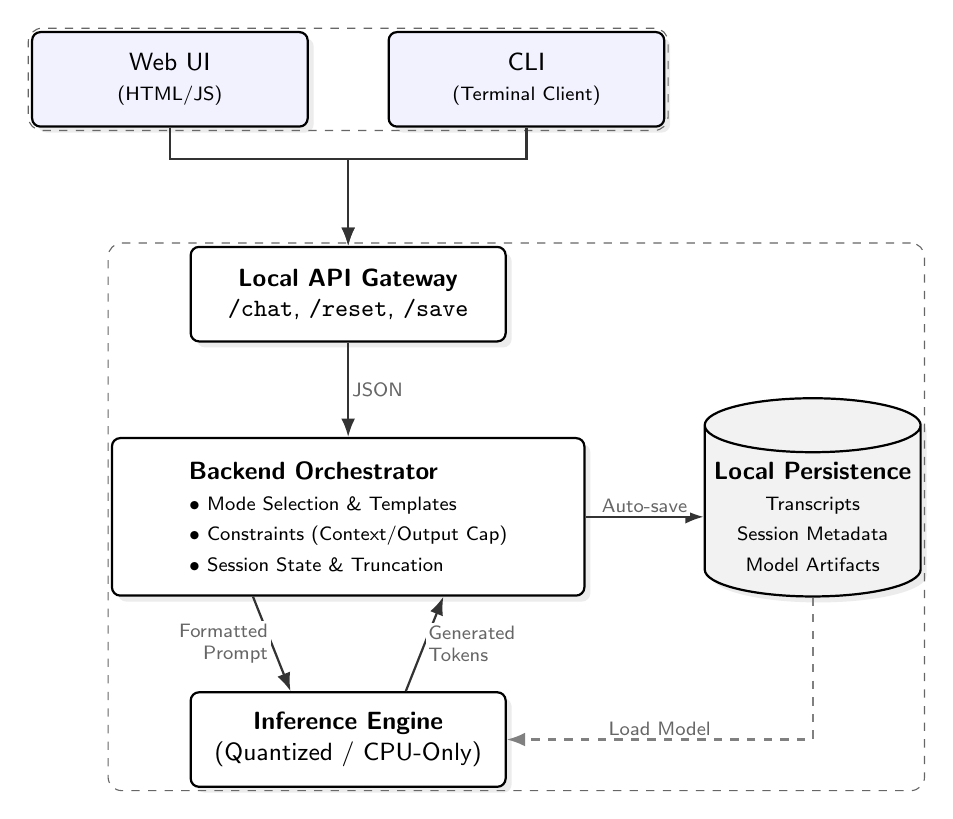
\begin{tikzpicture}[
    font=\sffamily\small,
    node distance=1.0cm and 1.0cm,
    % Styles
    process/.style={
        draw, fill=white, rounded corners=3pt, align=center, 
        minimum width=4cm, minimum height=1.2cm, 
        drop shadow={opacity=0.15}, thick
    },
    client/.style={
        draw, fill=blue!5, rounded corners=3pt, align=center, 
        minimum width=3.5cm, minimum height=1.2cm, 
        drop shadow={opacity=0.15}, thick
    },
    storage/.style={
        draw, cylinder, shape border rotate=90, aspect=0.25,
        fill=gray!10, align=center, 
        minimum width=2.5cm, minimum height=1.8cm, 
        drop shadow={opacity=0.15}, thick
    },
    container/.style={
        draw=gray!40, dashed, inner sep=12pt, rounded corners=5pt, fill=gray!3
    },
    arrow/.style={-Latex, thick, color=black!80},
    label/.style={font=\sffamily\scriptsize, color=black!60, fill=white, inner sep=1pt}
]

    % --- Clients ---
    \node[client] (web) {Web UI\\{\scriptsize (HTML/JS)}};
    \node[client, right=1.0cm of web] (cli) {CLI\\{\scriptsize (Terminal Client)}};

    % --- Application Layer ---
    \node[process, below=1.5cm of $(web.south)!0.5!(cli.south)$] (api) {
        \textbf{Local API Gateway}\\
        \texttt{/chat}, \texttt{/reset}, \texttt{/save}
    };

    \node[process, below=1.2cm of api, minimum width=6cm, minimum height=2cm, align=left] (backend) {
        \textbf{Backend Orchestrator}\\
        \scriptsize $\bullet$ Mode Selection \& Templates\\
        \scriptsize $\bullet$ Constraints (Context/Output Cap)\\
        \scriptsize $\bullet$ Session State \& Truncation
    };

    % --- Inference & Storage ---
    \node[process, below=1.2cm of backend] (engine) {
        \textbf{Inference Engine}\\
        (Quantized / CPU-Only)
    };

    \node[storage, right=1.5cm of backend] (store) {
        \textbf{Local Persistence}\\
        \scriptsize Transcripts\\
        \scriptsize Session Metadata\\
        \scriptsize Model Artifacts
    };

    % --- Connections ---
    % Clients to API
    \draw[arrow] (web.south) -- ++(0,-0.4) -| (api.north);
    \draw[arrow] (cli.south) -- ++(0,-0.4) -| (api.north);

    % API to Backend
    \draw[arrow] (api) -- node[right, label] {JSON} (backend);

    % Backend to Engine (Loop)
    \draw[arrow] (backend.220) -- node[left, label, align=right] {Formatted\\Prompt} (engine.140);
    \draw[arrow] (engine.40) -- node[right, label, align=left] {Generated\\Tokens} (backend.320);

    % Storage Interactions
    \draw[arrow] (backend.east) -- node[above, label] {Auto-save} (store.west);
    
    % Artifact loading (implied)
    \draw[arrow, dashed, gray] (store.south) |- node[pos=0.75, above, label] {Load Model} (engine.east);

    % --- Background Groups ---
    \begin{scope}[on background layer]
        \node[container, fit=(web) (cli), label={[anchor=north west]north west:\scriptsize \textbf{CLIENT LAYER}}] {};
        \node[container, fit=(api) (backend) (engine) (store), label={[anchor=north west]north west:\scriptsize \textbf{HOST SYSTEM (Local)}}] {};
    \end{scope}

\end{tikzpicture}
\caption{Pocket Brain technology-agnostic architecture, highlighting the separation between orchestration policy and raw inference.}
\end{figure}

\section{How ``Memory'' Works in Conversational LLMs (Key Concept)}
Large Language Models are \textbf{stateless} at inference time.
They do not store chat history internally between requests.
Conversational ``memory'' is implemented by the application layer by \textbf{resending prior turns} (a bounded subset of the transcript) along with the new user message on every request.

\subsection*{Implication}
Each new model call includes:
\begin{itemize}[leftmargin=*]
  \item System prompt (global behavior)
  \item Mode prompt (task framing)
  \item Selected conversation history (bounded window)
  \item Current user message
\end{itemize}
If the prompt exceeds the model's context window, the application must drop or compress older content.
Therefore, conversation continuity is a \textbf{systems policy decision}, not a property of the model.

\section{Resource Model: What Actually Consumes RAM}
On CPU-only inference, RAM usage is dominated by two primary components:
\begin{enumerate}[leftmargin=*]
  \item \textbf{Model weights:} quantization reduces memory footprint substantially (e.g., 4-bit weights vs 16-bit).
  \item \textbf{KV cache (context memory):} as context grows, the key/value cache grows, increasing working-set size and memory traffic.
\end{enumerate}

\subsection*{Why Context Management Matters}
Longer contexts expand the KV cache and increase memory bandwidth pressure.
This tends to reduce tokens-per-second and increase latency on CPU systems, especially as working sets exceed CPU cache and spill into main memory.
Pocket Brain therefore enforces \textbf{bounded context growth} and \textbf{bounded output length}.
While transcripts may be persisted to disk for long-term storage, only a limited working set is ever re-sent to the model. This distinction between persistent storage and active inference context is critical to maintaining predictable latency and memory usage under \(\leq\)8GB RAM.


\section{Context Management Policy (Pocket Brain Design)}
This section formalizes the policy you described (mode constraints + last \(N\) turns + new chat rollover + auto-save).

\subsection{Mode Scoping}
Pocket Brain enforces \textbf{one mode per session} (chat), selected at session creation.
Example modes:
\begin{itemize}[leftmargin=*]
  \item \texttt{perspectives}: generate alternative viewpoints and angles
  \item \texttt{risks}: identify weaknesses, failure modes, and unknowns
  \item \texttt{next\_steps}: produce actionable next actions and priorities
\end{itemize}
Rationale: mode scoping stabilizes behavior and reduces prompt bloat by avoiding multi-mode instruction stacking.

\subsection{Sliding Window History (Last \(N\) Exchanges)}
For each new request, Pocket Brain includes only the most recent \(N\) user-assistant exchanges (e.g., \(N=10\)).
Older content is not sent to the model for subsequent turns.
This bounded window provides conversational continuity while controlling KV cache growth.

\begin{figure}[h]
\centering
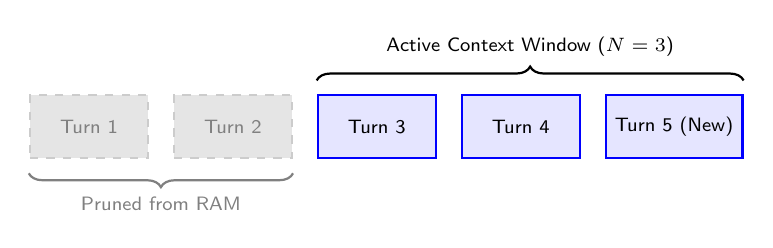
\begin{tikzpicture}[
    font=\sffamily\scriptsize,
    box/.style={draw, fill=white, minimum width=1.5cm, minimum height=0.8cm, thick},
    old/.style={box, fill=gray!20, draw=gray!40, dashed, text=gray},
    active/.style={box, fill=blue!10, draw=blue},
    arrow/.style={-Latex, thick}
]

% Timeline
\node[old] (t1) {Turn 1};
\node[old, right=0.3cm of t1] (t2) {Turn 2};
\node[active, right=0.3cm of t2] (t3) {Turn 3};
\node[active, right=0.3cm of t3] (t4) {Turn 4};
\node[active, right=0.3cm of t4] (t5) {Turn 5 (New)};

% Window Bracket
\draw[decoration={brace,amplitude=5pt,raise=5pt},decorate, thick]
  (t3.north west) -- node[above=10pt] {Active Context Window ($N=3$)} (t5.north east);

% Discarded Label
\draw[decoration={brace,amplitude=5pt,raise=5pt,mirror},decorate, thick, gray]
  (t1.south west) -- node[below=10pt] {Pruned from RAM} (t2.south east);

\end{tikzpicture}
\caption{Visualizing the sliding window policy. Older turns are persisted to disk but dropped from the active inference context.}
\end{figure}

\subsection{Explicit Session Rollover (``New Chat'')}
Pocket Brain supports a \textbf{New Chat} operation that:
\begin{itemize}[leftmargin=*]
  \item terminates the active session state,
  \item auto-saves the transcript to disk/SSD,
  \item creates a new session (optionally with a different mode).
\end{itemize}
This provides a simple and user-visible way to reset context and latency.

\subsection{Optional Hard Stop (optional session rollover limit)}
Some hosted systems stop a conversation after a usage threshold is reached.
Pocket Brain does \textbf{not} require a hard stop for technical correctness; truncation is sufficient.
However, an optional UX policy can be implemented:
\begin{itemize}[leftmargin=*]
  \item if repeated truncation is detected or the user reaches a configured turn limit,
  \item the UI suggests starting a new chat to preserve responsiveness,
  \item the system auto-saves and rolls over on user confirmation.
\end{itemize}

\begin{table}[h]
\centering
\small
\setlength{\tabcolsep}{8pt} % Increased padding
\renewcommand{\arraystretch}{1.4} % More breathing room
\begin{tabularx}{\textwidth}{@{} >{\bfseries}l l X @{}} % Bold first column, removal of side padding
\toprule
Parameter & Default (v1) & Rationale \\
\midrule
Mode per session & Fixed & Keeps prompts stable and avoids instruction stacking. \\
History window & Last \(N=10\) exchanges & Bounds KV cache growth to ensure predictable latency. \\
Output cap & Configurable max tokens & Prevents runaway responses on CPU. \\
New chat behavior & Auto-save then reset & Provides user-visible rollover and clear state. \\
Hard stop & Off by default & Truncation is sufficient; hard stop is optional UX. \\
\bottomrule
\end{tabularx}
\caption{Context management parameters for v1. Values may be tuned empirically once baseline performance is measured.}
\end{table}


\section{Model Candidates and Selection (v1)}

Pocket Brain does not train or fine-tune models.
Instead, it integrates existing open-weight, instruction-tuned language models that have been quantized for efficient CPU inference.
Model selection is driven by strict memory and latency constraints rather than benchmark maximization.

\subsection{Selection Criteria}
Candidate models must satisfy the following:
\begin{itemize}[leftmargin=*]
  \item Availability in GGUF or equivalent quantized format
  \item Stable CPU-only inference under \(\leq\)8GB RAM
  \item Instruction-tuned behavior suitable for conversational use
  \item Acceptable latency when context and output lengths are bounded
\end{itemize}

\subsection{Candidate Models}
Pocket Brain v1 considers the following models as viable options:

\begin{itemize}[leftmargin=*]
  \item \textbf{Qwen2.5 3B Instruct}:
  A strong default candidate offering balanced reasoning quality and efficiency for its size.
  Suitable for structured brainstorming tasks and mode-driven prompts.

  \item \textbf{Phi-2 / Phi-3 Mini}:
  Smaller, faster models well-suited for short-turn interactions and rapid iteration.
  These models trade some depth for lower latency and reduced memory pressure.

  \item \textbf{Mistral 7B Instruct}:
  A higher-capacity option reserved for deeper reasoning profiles.
  Use requires aggressive context and output caps to remain within memory constraints.
\end{itemize}

\begin{table}[h]
\centering
\small
\setlength{\tabcolsep}{5pt}
\renewcommand{\arraystretch}{1.3}
\begin{tabularx}{\textwidth}{@{} >{\bfseries}p{2.8cm} l l X l @{}} % Adjusted widths
\toprule
Model & Size & Target & Strengths for v1 & Role \\
\midrule
Qwen2.5 \newline Instruct & 3B & Q4/Q5 & Balanced quality/speed, strong instruction following. & \textbf{Default} \\
Phi-3 Mini & 3.8B & Q4/Q5 & Fast iteration, low memory pressure. & Alt-fast \\
Mistral Instruct & 7B & Q4 & Higher coherence, better complex reasoning. & Optional \\
\bottomrule
\end{tabularx}
\caption{Candidate models for Pocket Brain v1. Quantization targets are selected to maintain CPU-only feasibility under \(\leq\)8GB RAM.}
\end{table}



\subsection{Model Usage Strategy}
Pocket Brain v1 defaults to a \textbf{single-model strategy}, where interaction modes are implemented as prompt templates rather than model switching.
This approach minimizes operational complexity and preserves consistent behavior across sessions.

Support for multiple models (e.g., a ``fast'' and ``deep'' profile) is considered a future extension and is not required for v1.


\section{API-Level Feature Set (Driven by Clients)}
The Web UI and CLI are thin clients; all core policies live server-side.
The minimal API features required to support the memory and mode behavior above are:
\begin{itemize}[leftmargin=*]
  \item \textbf{Create session:} establish \texttt{session\_id} and fixed \texttt{mode}
  \item \textbf{Chat:} submit a message, return assistant output
  \item \textbf{Reset / New chat:} clear session state and/or create a new session
  \item \textbf{Save:} persist transcript to disk/SSD
  \item \textbf{Health/status:} confirm model loaded and service operational
\end{itemize}

\section{Technology Option Sets (Top 3 per Component)}
\vspace{-10pt}
\begin{figure}[h]
\centering
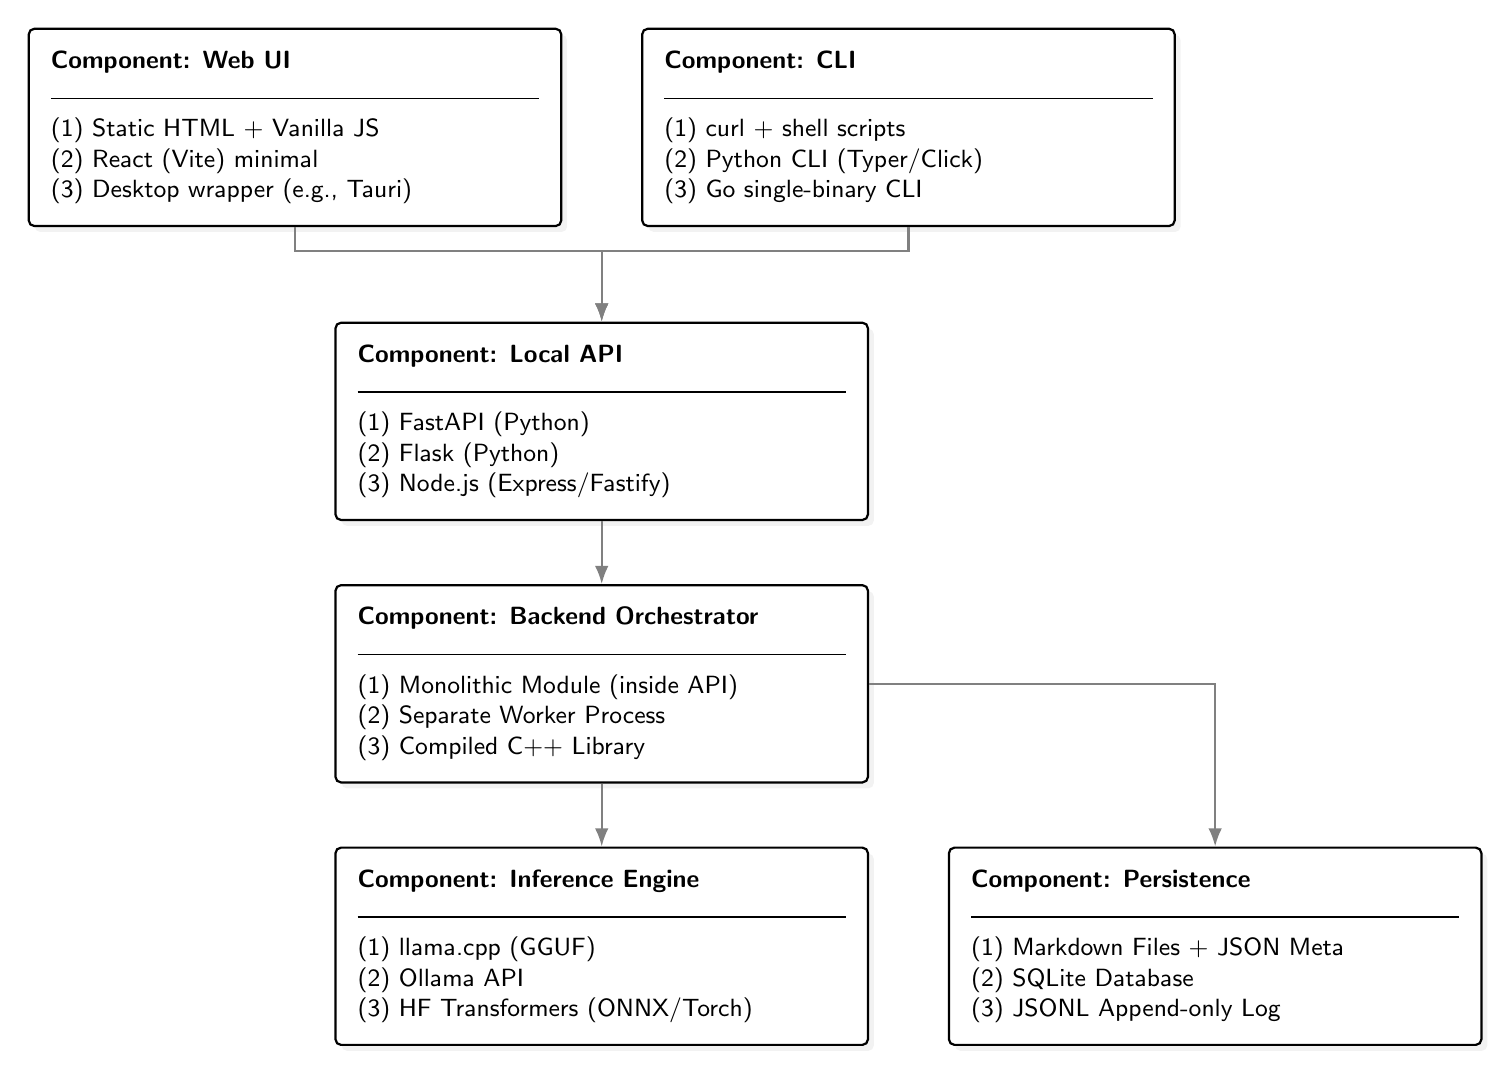
\begin{tikzpicture}[
    font=\sffamily\small,
    node distance=0.9cm,
    % Styles
    optionbox/.style={
        draw, fill=white, rounded corners=2pt, align=left, 
        minimum width=6.5cm, inner sep=8pt,
        drop shadow={opacity=0.1}, thick
    },
    header/.style={
        font=\bfseries, align=center, minimum width=6.5cm, 
        yshift=-10pt
    },
    arrow/.style={-Latex, thick, gray}
]

    % --- Row 1: Clients ---
    \node[optionbox] (web) {
        \textbf{Component: Web UI}\\
        \rule{6.2cm}{0.4pt}\\[0.3em]
        (1) Static HTML + Vanilla JS\\
        (2) React (Vite) minimal\\
        (3) Desktop wrapper (e.g., Tauri)
    };

    \node[optionbox, right=1cm of web] (cli) {
        \textbf{Component: CLI}\\
        \rule{6.2cm}{0.4pt}\\[0.3em]
        (1) curl + shell scripts\\
        (2) Python CLI (Typer/Click)\\
        (3) Go single-binary CLI
    };

    % --- Row 2: API ---
    \node[optionbox, below=1.2cm of $(web.south)!0.5!(cli.south)$] (api) {
        \textbf{Component: Local API}\\
        \rule{6.2cm}{0.4pt}\\[0.3em]
        (1) FastAPI (Python)\\
        (2) Flask (Python)\\
        (3) Node.js (Express/Fastify)
    };

    % --- Row 3: Orchestrator ---
    \node[optionbox, below=0.8cm of api] (backend) {
        \textbf{Component: Backend Orchestrator}\\
        \rule{6.2cm}{0.4pt}\\[0.3em]
        (1) Monolithic Module (inside API)\\
        (2) Separate Worker Process\\
        (3) Compiled C++ Library
    };

    % --- Row 4: Engine & Storage ---
    \node[optionbox, below=0.8cm of backend] (engine) {
        \textbf{Component: Inference Engine}\\
        \rule{6.2cm}{0.4pt}\\[0.3em]
        (1) llama.cpp (GGUF)\\
        (2) Ollama API\\
        (3) HF Transformers (ONNX/Torch)
    };

    \node[optionbox, right=1cm of engine, align=left] (store) {
        \textbf{Component: Persistence}\\
        \rule{6.2cm}{0.4pt}\\[0.3em]
        (1) Markdown Files + JSON Meta\\
        (2) SQLite Database\\
        (3) JSONL Append-only Log
    };

    % --- Connections ---
    \draw[arrow] (web.south) -- ++(0,-0.3) -| (api.north);
    \draw[arrow] (cli.south) -- ++(0,-0.3) -| (api.north);
    \draw[arrow] (api) -- (backend);
    \draw[arrow] (backend) -- (engine);
    \draw[arrow] (backend.east) -| (store.north);

\end{tikzpicture}
\caption{Constrained technology option sets. The modular architecture allows swapping components (e.g., replacing Flask with FastAPI) without redesigning the system.}
\end{figure}

\newpage
\section{Deliverables and Milestones (Implementation Plan)}
\subsection*{Milestone 1: End-to-End Skeleton}
\begin{itemize}[leftmargin=*]
  \item API service running locally
  \item Session creation, chat request, and response
  \item Auto-save transcript to disk on demand
\end{itemize}

\subsection*{Milestone 2: Enforced Constraints}
\begin{itemize}[leftmargin=*]
  \item Fixed mode per session
  \item Sliding window history (last \(N\) exchanges)
  \item Output caps (max tokens) and context caps
\end{itemize}

\subsection*{Milestone 3: Usability}
\begin{itemize}[leftmargin=*]
  \item Web UI and CLI client parity
  \item ``New Chat'' rollover and clear chat controls
  \item Health/status endpoint + basic logging
\end{itemize}

\begin{table}[h]
\centering
\footnotesize % Slightly smaller font to fit comfortably
\setlength{\tabcolsep}{4pt}
\renewcommand{\arraystretch}{1.5}
\begin{tabularx}{\textwidth}{@{} >{\bfseries}p{2.5cm} X X X c @{}}
\toprule
Component & Option 1 & Option 2 & Option 3 & \textbf{Select} \\
\midrule
Web UI & Static HTML + JS & React (Vite) & Tauri wrapper & TBD \\
CLI & curl + shell & Python (Typer) & Go CLI & TBD \\
Local API & FastAPI & Flask & Node (Express) & TBD \\
Orchestrator & In-API Module & Worker process & C++ Lib & TBD \\
Engine & llama.cpp (GGUF) & Ollama & Torch/ONNX & TBD \\
Persistence & Markdown/JSON & SQLite & JSONL Log & TBD \\
\bottomrule
\end{tabularx}
\caption{Technology decision matrix. The selection will be finalized based on v1 implementation constraints.}
\end{table}

\newpage

\section{Versioning and Planned Evolution}

\subsection*{Version 1 (Current Scope)}
Pocket Brain v1 focuses on:
\begin{itemize}[leftmargin=*]
  \item text-only interaction,
  \item a single quantized model,
  \item fixed interaction modes per session,
  \item sliding window context truncation,
  \item local persistence of transcripts.
\end{itemize}

\subsection*{Potential Future Extensions}
Future versions may explore:
\begin{itemize}[leftmargin=*]
  \item multi-profile inference (fast vs deep),
  \item improved launchers for Windows and macOS,
  \item optional import/export tooling,
  \item limited multimodal extensions.
\end{itemize}

These extensions are intentionally excluded from v1 to preserve clarity, stability, and bounded complexity.


\section{Non-Goals}
Pocket Brain explicitly excludes:
\begin{itemize}[leftmargin=*]
  \item model training or fine-tuning,
  \item long-document ingestion or RAG in v1,
  \item multi-user authentication and cloud deployment,
  \item GPU acceleration requirements.
\end{itemize}

\section{Conclusion}
Pocket Brain v1 demonstrates that a useful conversational assistant can be built under strict CPU-only and memory-constrained conditions by treating context management and interaction design as first-class systems problems.
Rather than maximizing model size or feature count, the system emphasizes bounded resource usage, predictable latency, and structured prompting.
This approach enables private, offline brainstorming workflows while remaining transparent, portable, and technically tractable.

\end{document}
